%% BioMed_Central_Tex_Template_v1.06
%%                                      %
%  bmc_article.tex            ver: 1.06 %
%                                       %

%%IMPORTANT: do not delete the first line of this template
%%It must be present to enable the BMC Submission system to 
%%recognise this template!!

%%%%%%%%%%%%%%%%%%%%%%%%%%%%%%%%%%%%%%%%%
%%                                     %%
%%  LaTeX template for BioMed Central  %%
%%     journal article submissions     %%
%%                                     %%
%%         <14 August 2007>            %%
%%                                     %%
%%                                     %%
%% Uses:                               %%
%% cite.sty, url.sty, bmc_article.cls  %%
%% ifthen.sty. multicol.sty     		   %%
%%				      	                     %%
%%                                     %%
%%%%%%%%%%%%%%%%%%%%%%%%%%%%%%%%%%%%%%%%%


%%%%%%%%%%%%%%%%%%%%%%%%%%%%%%%%%%%%%%%%%%%%%%%%%%%%%%%%%%%%%%%%%%%%%
%%                                                                 %%	
%% For instructions on how to fill out this Tex template           %%
%% document please refer to Readme.pdf and the instructions for    %%
%% authors page on the biomed central website                      %%
%% http://www.biomedcentral.com/info/authors/                      %%
%%                                                                 %%
%% Please do not use \input{...} to include other tex files.       %%
%% Submit your LaTeX manuscript as one .tex document.              %%
%%                                                                 %%
%% All additional figures and files should be attached             %%
%% separately and not embedded in the \TeX\ document itself.       %%
%%                                                                 %%
%% BioMed Central currently use the MikTex distribution of         %%
%% TeX for Windows) of TeX and LaTeX.  This is available from      %%
%% http://www.miktex.org                                           %%
%%                                                                 %%
%%%%%%%%%%%%%%%%%%%%%%%%%%%%%%%%%%%%%%%%%%%%%%%%%%%%%%%%%%%%%%%%%%%%%


\NeedsTeXFormat{LaTeX2e}[1995/12/01]
\documentclass[10pt]{bmc_article}    



% Load packages
\usepackage{cite} % Make references as [1-4], not [1,2,3,4]
\usepackage{url}  % Formatting web addresses  
\usepackage{ifthen}  % Conditional 
\usepackage{multicol}   %Columns
\usepackage[utf8]{inputenc} %unicode support
%\usepackage[applemac]{inputenc} %applemac support if unicode package fails
%\usepackage[latin1]{inputenc} %UNIX support if unicode package fails
\usepackage{graphicx}
\urlstyle{rm}
 
 
%%%%%%%%%%%%%%%%%%%%%%%%%%%%%%%%%%%%%%%%%%%%%%%%%	
%%                                             %%
%%  If you wish to display your graphics for   %%
%%  your own use using includegraphic or       %%
%%  includegraphics, then comment out the      %%
%%  following two lines of code.               %%   
%%  NB: These line *must* be included when     %%
%%  submitting to BMC.                         %% 
%%  All figure files must be submitted as      %%
%%  separate graphics through the BMC          %%
%%  submission process, not included in the    %% 
%%  submitted article.                         %% 
%%                                             %%
%%%%%%%%%%%%%%%%%%%%%%%%%%%%%%%%%%%%%%%%%%%%%%%%%                     


\def\includegraphic{}
\def\includegraphics{}



\setlength{\topmargin}{0.0cm}
\setlength{\textheight}{21.5cm}
\setlength{\oddsidemargin}{0cm} 
\setlength{\textwidth}{16.5cm}
\setlength{\columnsep}{0.6cm}

\newboolean{publ}

%%%%%%%%%%%%%%%%%%%%%%%%%%%%%%%%%%%%%%%%%%%%%%%%%%
%%                                              %%
%% You may change the following style settings  %%
%% Should you wish to format your article       %%
%% in a publication style for printing out and  %%
%% sharing with colleagues, but ensure that     %%
%% before submitting to BMC that the style is   %%
%% returned to the Review style setting.        %%
%%                                              %%
%%%%%%%%%%%%%%%%%%%%%%%%%%%%%%%%%%%%%%%%%%%%%%%%%%
 

%Review style settings
\newenvironment{bmcformat}{\begin{raggedright}\baselineskip20pt\sloppy\setboolean{publ}{false}}{\end{raggedright}\baselineskip20pt\sloppy}

%Publication style settings
%\newenvironment{bmcformat}{\fussy\setboolean{publ}{true}}{\fussy}



% Begin ...
\begin{document}
\begin{bmcformat}


%%%%%%%%%%%%%%%%%%%%%%%%%%%%%%%%%%%%%%%%%%%%%%
%%                                          %%
%% Enter the title of your article here     %%
%%                                          %%
%%%%%%%%%%%%%%%%%%%%%%%%%%%%%%%%%%%%%%%%%%%%%%

\title{Identification of structural classes in metabolomics}

%%%%%%%%%%%%%%%%%%%%%%%%%%%%%%%%%%%%%%%%%%%%%%
%%                                          %%
%% Enter the authors here                   %%
%%                                          %%
%% Ensure \and is entered between all but   %%
%% the last two authors. This will be       %%
%% replaced by a comma in the final article %%
%%                                          %%
%% Ensure there are no trailing spaces at   %% 
%% the ends of the lines                    %%     	
%%                                          %%
%%%%%%%%%%%%%%%%%%%%%%%%%%%%%%%%%%%%%%%%%%%%%%


\author{Pablo A Moreno\correspondingauthor$^1$%
       \email{Pablo A Moreno\correspondingauthor - pmoreno@ebi.ac.uk}%
	 \and
	 Steffen Neumann$^1$
	 \email{Steffen Neumann\correspondingauthor - sneumann@ipb-halle.de}%
       and 
         Christoph Steinbeck$^1$%
         \email{Christoph Steinbeck\correspondingauthor - steinbeck@ebi.ac.uk}%
      }
      

%%%%%%%%%%%%%%%%%%%%%%%%%%%%%%%%%%%%%%%%%%%%%%
%%                                          %%
%% Enter the authors' addresses here        %%
%%                                          %%
%%%%%%%%%%%%%%%%%%%%%%%%%%%%%%%%%%%%%%%%%%%%%%

\address{%
    \iid(1)Chemoinformatics and Metabolism Team, European Bioinformatics Institute (EBI), Cambridge, UK\\
    \iid(2)Massspectrometry and Bioinformatics Group, Institute for Plant Biochemistry (IPB), Halle, Germany
}%

\maketitle

%%%%%%%%%%%%%%%%%%%%%%%%%%%%%%%%%%%%%%%%%%%%%%
%%                                          %%
%% The Abstract begins here                 %%
%%                                          %%
%% The Section headings here are those for  %%
%% a Research article submitted to a        %%
%% BMC-Series journal.                      %%  
%%                                          %%
%% If your article is not of this type,     %%
%% then refer to the Instructions for       %%
%% authors on http://www.biomedcentral.com  %%
%% and change the section headings          %%
%% accordingly.                             %%   
%%                                          %%
%%%%%%%%%%%%%%%%%%%%%%%%%%%%%%%%%%%%%%%%%%%%%%


\begin{abstract}
        % Do not use inserted blank lines (ie \\) until main body of text.
        \paragraph*{Background:} The identification of metabolites in metabolomics and natural products research
based on their spectral and chromatographic properties is a multi-layered process, where one first aims to find the correct compound
by spectral library searches. If this is unsuccessful, de-novo structure elucidation is in order. The success of this potentially complex process is strongly influenced by the choice of a good hypothetical starting structure. 
      
        \paragraph*{Results:} Here we present the combination of XXX with the ChEBI ontology to calculate ontology enrichments ... XXX

        \paragraph*{Conclusions:} We have shown that ... XXXX ... leads to ....XXX ...
\end{abstract}



\ifthenelse{\boolean{publ}}{\begin{multicols}{2}}{}




%%%%%%%%%%%%%%%%%%%%%%%%%%%%%%%%%%%%%%%%%%%%%%
%%                                          %%
%% The Main Body begins here                %%
%%                                          %%
%% The Section headings here are those for  %%
%% a Research article submitted to a        %%
%% BMC-Series journal.                      %%  
%%                                          %%
%% If your article is not of this type,     %%
%% then refer to the instructions for       %%
%% authors on:                              %%
%% http://www.biomedcentral.com/info/authors%%
%% and change the section headings          %%
%% accordingly.                             %% 
%%                                          %%
%% See the Results and Discussion section   %%
%% for details on how to create sub-sections%%
%%                                          %%
%% use \cite{...} to cite references        %%
%%  \cite{koon} and                         %%
%%  \cite{oreg,khar,zvai,xjon,schn,pond}    %%
%%  \nocite{smith,marg,hunn,advi,koha,mouse}%%
%%                                          %%
%%%%%%%%%%%%%%%%%%%%%%%%%%%%%%%%%%%%%%%%%%%%%%




%%%%%%%%%%%%%%%%
%% Background %%
%%
\section*{Background}

Lorem ipsum dolor sit amet, consectetur adipiscing elit. Nullam vel mauris et eros convallis mollis. Nullam at purus et massa aliquet consequat elementum tincidunt leo. Proin tristique, felis in lobortis accumsan, erat magna faucibus nulla, ac ornare ipsum tellus in metus. Suspendisse dui arcu, dapibus nec consequat eu, commodo non arcu. Aenean ultrices massa quis sem egestas quis feugiat orci rhoncus. Pellentesque elementum lorem ac tellus imperdiet in porttitor felis hendrerit. Suspendisse potenti. Ut quis mi non diam adipiscing sollicitudin. Nullam id consectetur nibh. Pellentesque imperdiet velit sit amet odio mattis ultricies. Mauris gravida orci a sem vehicula et semper augue hendrerit. Sed at pulvinar felis. Mauris tincidunt molestie nulla, eget condimentum purus condimentum id. Aenean mauris neque, dapibus vel sagittis vel, semper quis libero. Praesent malesuada massa sit amet felis ultrices molestie. Proin tempor commodo varius. Etiam at nisl eu ante porta consequat nec nec quam. Cras molestie quam vitae risus ullamcorper quis porttitor mi fringilla.

%%%%%%%%%%%%%%%%%%
\section*{Methods}

Action items:

1) Steffen: make MetFrag work against ChEBI

2) Steffen/Pablo: calculate the most general ChEBI ID
 from the 300 compounds, ignoring stereo

3) Pablo: make a batch version of the overrepresentation analysis 
 of ChEBI IDs. Question: Output format ? PDF ? SVG ? Cytoscape ?

4) Steffen: run our MetFrag benchmark against ChEBI
 Output format: 300 CSV files "score, ChEBI-ID" 
 with the ID of the correct compound in the filename.

5) Pablo/Christoph/Steffen: 
 Discuss whether we a) need to postprocess the network at all, 
 and if so b) how, to obtain more disjoint "answers" 
 from the ontology.

6) Steffen: calculate the MetFrag/ChEBI results 
 in terms of "correct/max/avg rank"

Mauris bibendum feugiat enim ut ultrices. Vestibulum varius laoreet dolor eget ultrices. Sed in massa vitae lorem egestas hendrerit. Duis interdum sapien a purus porta consectetur. Donec non nunc tortor. Suspendisse aliquet consectetur quam, at pharetra nulla hendrerit nec. Etiam mauris augue, lobortis ut vestibulum nec, aliquam eu ipsum. Vivamus eget nisi lacus, ut blandit felis. Nunc laoreet commodo condimentum. Nullam interdum, sapien nec lobortis ornare, eros tortor molestie velit, sed imperdiet neque dolor a lacus.

\subsection*{Requirements}

Praesent neque lorem, adipiscing in fermentum vitae, iaculis gravida ipsum. Sed eleifend pellentesque faucibus. Nulla convallis, risus et fringilla tempor, tortor velit sagittis sem, a accumsan mi lacus eget sem. Etiam neque diam, iaculis non ornare at, tincidunt non nunc. Integer pellentesque viverra libero in semper. Vivamus non hendrerit est. Pellentesque elementum ante eu erat ultricies posuere. Donec non turpis neque, id mattis tortor. Donec pellentesque ultrices tortor vitae ultrices. Ut ac urna a sem convallis pretium. Nam et eros vestibulum orci eleifend viverra. Fusce pulvinar gravida sem in ultrices. Vestibulum porttitor hendrerit ipsum. Aliquam erat volutpat. Praesent lectus nisi, vestibulum ac consequat eu, malesuada tincidunt massa. Sed aliquet luctus ante in varius.

%%%%%%%%%%%%%%%%%%%%%%%%%%%%
%% Results and Discussion %%
%%
\section*{Results and Discussion}

Lorem ipsum dolor sit amet, consectetur adipiscing elit. Nullam vel mauris et eros convallis mollis. Nullam at purus et massa aliquet consequat elementum tincidunt leo. Proin tristique, felis in lobortis accumsan, erat magna faucibus nulla, ac ornare ipsum tellus in metus. Suspendisse dui arcu, dapibus nec consequat eu, commodo non arcu. Aenean ultrices massa quis sem egestas quis feugiat orci rhoncus. Pellentesque elementum lorem ac tellus imperdiet in porttitor felis hendrerit. Suspendisse potenti. Ut quis mi non diam adipiscing sollicitudin. Nullam id consectetur nibh. Pellentesque imperdiet velit sit amet odio mattis ultricies. Mauris gravida orci a sem vehicula et semper augue hendrerit. Sed at pulvinar felis. Mauris tincidunt molestie nulla, eget condimentum purus condimentum id. Aenean mauris neque, dapibus vel sagittis vel, semper quis libero. Praesent malesuada massa sit amet felis ultrices molestie. Proin tempor commodo varius. Etiam at nisl eu ante porta consequat nec nec quam. Cras molestie quam vitae risus ullamcorper quis porttitor mi fringilla.

%%%%%%%%%%%%%%%%%%%%%%
\section*{Conclusions}
Ut quis massa non ligula aliquam rhoncus vitae non ante. Pellentesque ante elit, interdum vitae rutrum id, fermentum eget eros. Mauris in quam nunc, in auctor sapien. In molestie eros et massa pellentesque et ultricies lectus porttitor. Pellentesque sollicitudin, sapien sit amet porttitor bibendum, odio libero tincidunt eros, et vehicula ante neque ac nisi. Nam mollis elit at ante convallis rutrum. Morbi a diam urna, vel sollicitudin lorem. Fusce laoreet, metus ac hendrerit sollicitudin, eros orci tempus elit, a vulputate lorem justo vel metus. Proin aliquam nulla nec velit interdum porttitor. Cras et massa augue, molestie aliquam nulla. Mauris magna leo, molestie sit amet congue fermentum, dapibus et leo. Vivamus eu lacus vestibulum ligula ornare lobortis vitae at ipsum. Nunc vulputate gravida dui imperdiet laoreet.

    
%%%%%%%%%%%%%%%%%%%%%%%%%%%%%%%%
\section*{Authors contributions}
SN, PM and CS conceived the project, and lead the further development. 
SN worked on MetFrag-ChEBI integration 
PM worked on the ontology enrichment 
All co-authors contributed to the manuscript. 
All authors read and approved the final manuscript.
	    

%%%%%%%%%%%%%%%%%%%%%%%%%%%
\section*{Acknowledgements}
  \ifthenelse{\boolean{publ}}{\small}{}


 
%%%%%%%%%%%%%%%%%%%%%%%%%%%%%%%%%%%%%%%%%%%%%%%%%%%%%%%%%%%%%
%%                  The Bibliography                       %%
%%                                                         %%              
%%  Bmc_article.bst  will be used to                       %%
%%  create a .BBL file for submission, which includes      %%
%%  XML structured for BMC.                                %%
%%  After submission of the .TEX file,                     %%
%%  you will be prompted to submit your .BBL file.         %%
%%                                                         %%
%%                                                         %%
%%  Note that the displayed Bibliography will not          %% 
%%  necessarily be rendered by Latex exactly as specified  %%
%%  in the online Instructions for Authors.                %% 
%%                                                         %%
%%%%%%%%%%%%%%%%%%%%%%%%%%%%%%%%%%%%%%%%%%%%%%%%%%%%%%%%%%%%%


{\ifthenelse{\boolean{publ}}{\footnotesize}{\small}
 \bibliographystyle{bmc_article}  % Style BST file
  \bibliography{bmc_article} }     % Bibliography file (usually '*.bib' ) 

%%%%%%%%%%%

\ifthenelse{\boolean{publ}}{\end{multicols}}{}

%%%%%%%%%%%%%%%%%%%%%%%%%%%%%%%%%%%
%%                               %%
%% Figures                       %%
%%                               %%
%% NB: this is for captions and  %%
%% Titles. All graphics must be  %%
%% submitted separately and NOT  %%
%% included in the Tex document  %%
%%                               %%
%%%%%%%%%%%%%%%%%%%%%%%%%%%%%%%%%%%

%%
%% Do not use \listoffigures as most will included as separate files

\section*{Figures} 
\begin{figure*}[hbt]
  \centering
	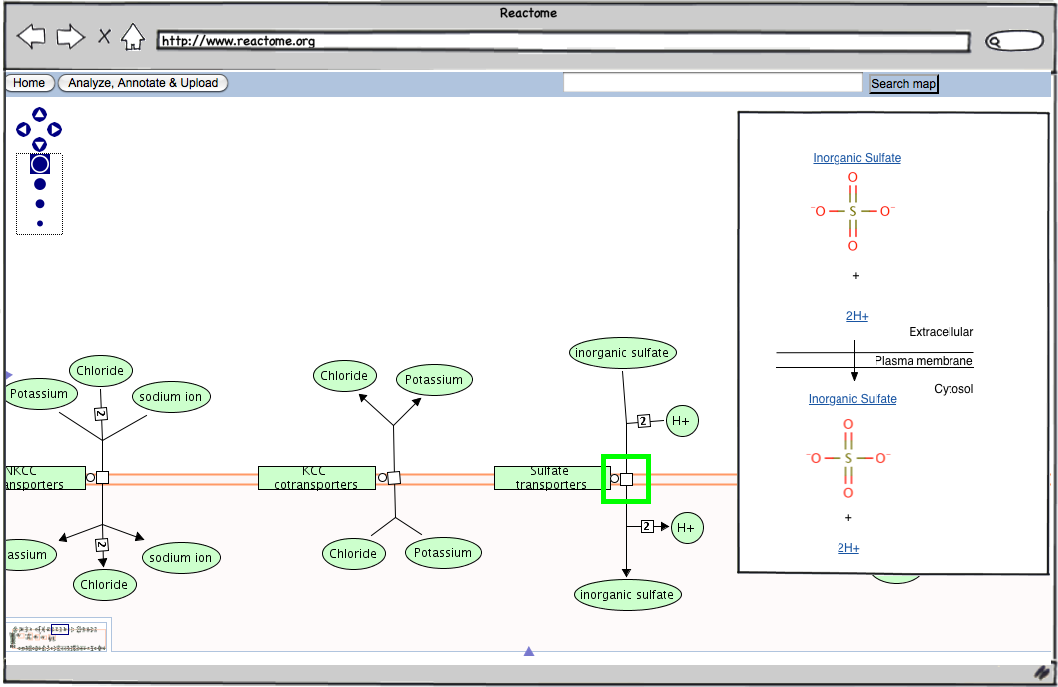
\includegraphics[angle=0,clip=false,scale=1.0]{pics/pathwayPopUpTransport.png}
  \caption{Lorem ipsum}
  \label{fig:ReactionEnumerationWorkflow}
\end{figure*}



%%%%%%%%%%%%%%%%%%%%%%%%%%%%%%%%%%%
%%                               %%
%% Tables                        %%
%%                               %%
%%%%%%%%%%%%%%%%%%%%%%%%%%%%%%%%%%%

%% Use of \listoftables is discouraged.
%%
\section*{Tables}
  \subsection*{Table 1 - Stuff in Tables}
    Overview on Stuff in Tables \par \mbox{}
    \par
    \mbox{
      \begin{tabular}{|c|c|c|}\hline 
        \textbf{Function} &  \textbf{\# workers}  & \textbf{Examples} \\ \hline
        File I/O & ?  & SDFReader, InChIReader \\ \hline
        Molecular descriptor calculation & ? & AtomCount, LargestChain, WienerIndex \\ \hline
        Machine learning & ?  & kMeans, Perceptron, SVM  \\ \hline
      \end{tabular}
      }


\end{bmcformat}
\end{document}







